\def\tutdate{17.01.2018}

\documentclass{beamer}
\usepackage{../templates/beamerthemekitwide}
%\usepackage{enumitem}

\usepackage[utf8]{inputenc}
\usepackage[T1]{fontenc}
\usepackage[ngerman]{babel}
\usepackage{listings}
\usepackage{hyperref}
\usepackage{graphicx}

\usepackage{amsmath}
\usepackage{amsthm}
\usepackage{amssymb}
\usepackage{polynom}

%\usepackage{ifthen}
%\usepackage{adjustbox} % for \adjincludegraphics

%\usepackage{tikz}
\usepackage{listings}

%\usepackage[]{algorithm2e}

%\usepackage{colortbl}
\usepackage{verbatim}
%\usepackage{alltt}
%\usepackage{changes}

%\usepackage{pdfpages}
%\usepackage{tabularx}

%\usepackage{euler}


\newcommand{\markBlue}[1]{\textcolor{kit-blue100}{#1}}
\newcommand{\markGreen}[1]{\textcolor{kit-green100}{#1}}
\newcommand{\vertspace}{\vspace{.2cm}}

%\newcommand{\#}{\markBlue{#1}}

%\newcommand{\pitem}{\pause\item}
\newcommand{\p}{\pause}

% -- MATH MACROS
\newcommand{\thistheoremname}{}
\newcommand{\G}{\mathbb{Z}}
\newcommand{\B}{\mathbb{B}}
\newcommand{\R}{\mathbb{R}}
\newcommand{\N}{\mathbb{N}}
\newcommand{\Q}{\mathbb{Q}}
\newcommand{\C}{\mathbb{C}}
\newcommand{\Z}{\mathbb{Z}}
\newcommand{\F}{\mathbb{F}}
\newcommand{\mi}{\mathrm{i}}
\renewcommand{\epsilon}{\varepsilon}
\newcommand{\okalk}{\mathscr{O}}


\newenvironment<>{taskblock}[1]{%
	\setbeamercolor{block title}{fg=kit-orange15,bg=kit-orange100}
	\setbeamercolor{block body}{fg=black,bg=kit-orange30}%
	\begin{block}#2{#1}}{\end{block}}

\setbeamertemplate{enumerate items}[default]

% Aussagenlogik Symbole
\newcommand{\W}{w}
\renewcommand{\F}{f}

% Kodierung
\newcommand{\frepr}{\textbf{repr}}
\newcommand{\fRepr}{\textbf{Repr}}
\newcommand{\fZkpl}{\textbf{Zkpl}}
\newcommand{\fbin}{\textbf{bin}}
\newcommand{\fdiv}{\textbf{ div }}
\newcommand{\fmod}{\textbf{ mod }}

% Speicherabbild
\newenvironment{memory}{\begin{tabular}{r | l}Adresse&Wert\\\hline\hline}{\end{tabular}}
\newcommand{\memrow}[2]{#1 & #2 \\\hline}

% Praedikatenlogik
\newcommand{\objequiv}{\stackrel{\cdot}{=}}
\newcommand{\pval}{val_{D,I,\beta}}

% Neue Befehle
\newcommand{\ip}{\pause} % inline pause, für mitten im satz
\newcommand{\pitem}{\pause\item} % für aufzählungen
\newcommand{\bp}{\pause} % block pause, für zwischen blöcken
\title[Grundbegriffe der Informatik]{ICPC\\Gruppe 2}
\date{\tutdate}
\subtitle{\tutTitle}
\author{Elias Schaut, Dennis Kobert, Niklas Kniep, Lam Vo, Ilia Bozhinov}

\institute{}

\titleimage{bg}
%\titleimage{bg-advent}

%
\ifthenelse{\equal{\compiletype}{livebeamer}}
	{
		\def\livebeamermode{1}
	}{}

\ifthenelse{\equal{\compiletype}{print}}
	{
		\def\printmode{1}
	}{}

\setbeamercovered{invisible}

%\usepackage[citestyle=authoryear,bibstyle=numeric,hyperref,backend=biber]{biblatex}
%\addbibresource{templates/example.bib}
%\bibhang1em

	
\def\tutTitle{O-Kalkül und Mastertheorem}
\begin{document}

\selectlanguage{ngerman}

%title page
\begin{frame}
	\titlepage
\end{frame}

\section{Komplexitätstheorie}
\begin{frame}{Rückblick}
	\begin{itemize}
		\pitem Was ist $\Omega(f), \Theta(f), \okalk(f)$?
		\pitem Wieso messen wir nicht einfach Laufzeit in ``Anzahl Operationen''?
	\end{itemize}
\end{frame}

\begin{frame}{Obere und untere Schranke}
	\begin{block}{Obere Schranke (Worst-Case Approximation)}
		$O(f) = \{g| \exists c \in \mathbb{R}_+ : \exists n_0 \in \mathbb{N}_0: \forall n \geq n_0 : g(n)\leq c \cdot f(n)\}$
	\end{block}
	
	\pause
	
	\begin{block}{Untere Schranke (Best-Case Approximation)}
		$\Omega(f) = \{g| \exists c \in \mathbb{R}_+ : \exists n_0 \in \mathbb{N}_0: \forall n \geq n_0 : g(n)\geq c \cdot f(n)\}$
	\end{block}

	\pause

	\begin{block}{Average-Case Approximation}
		$\Theta(f) = \{g|\exists c, c' \in \mathbb{R}_+ : \exists n_0 \in \mathbb{N}_0: \forall n \geq n_0 : c \cdot f(n) \leq g(n)\leq c' \cdot f(n)\}$
	\end{block}

	\pause
	
\end{frame}

\begin{frame}{Wiederholung}
Ist die Aussage wahr?
\begin{itemize}
\pitem $\pi n^{10} \in O(\frac{1}{e^{10}} n^{10})$ \pause Ja
\pitem $5n^2+3 \in O(\frac{1}{2}n^2)$ \pause Ja
\pitem $5^n \in O(3^n)$ \pause Nein
\pitem $\log_3(n^2) \in O(7\log_2(n))$ \pause Ja
\pitem $n^n \in O(n!)$ \pause Nein

\end{itemize}

\end{frame}

\begin{frame}{Aufgabe}
	Zeige, dass $f(n) \in \Theta(g(n))$ mit $f(n)=2n^4+4n^3$ und $g(n)=5n^4-2n^2$
\end{frame}

\begin{frame}
	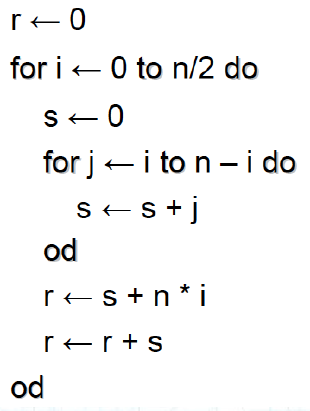
\includegraphics[scale=0.5]{images/okalk_algo.png}
	
	\begin{itemize}
		\pitem Wie oft wird die innere Schleife durchlaufen? \pause $n-2i+1$ mal.
		\pitem Wie kommen wir jetzt auf die Gesamtlaufzeit?
		\pitem $\sum\limits_{i=0}^{n/2} (n-2i+1) \ip = \frac{n}{2}n -2\sum\limits_{i=0}^{n/2}i+\frac{n}{2} \ip = \frac{n^2}{2}+\frac{n}{2}-2\frac{\frac{n}{2}\cdot \left(\frac{n}{2}+1\right)}{2} \ip = \frac{n^2}{2}+\frac{n}{2}-\frac{n^2}{4}-\frac{n}{2}\ip = \frac{1}{4}n^2$
	\end{itemize}
\end{frame}


\subsection{Mastertheorem}

\begin{frame}{Mastertheorem}
	\begin{block}{Formel für Mastertheorem}
		Rekursive Komplexitätsformeln der Form\\
		
		\vspace{.2cm}
		$\quad T(n) = a \cdot T(\frac{n}{b}) + f(n)$
		\vspace{.2cm}
		
		lassen sich mit dem Mastertheorem Komplexitätsklassen zuordnen.
	\end{block}

	\begin{block}{Auflösung des Mastertheorem}
		\begin{description}
			\item[Fall 1:] Wenn $f \in \okalk(n^{\log_b a -\epsilon})$ für ein
			$\epsilon>0$ ist, dann ist $T\in \Theta(n^{\log_b a})$.
			\item[Fall 2:] Wenn $f \in \Theta(n^{\log_b a})$ ist, dann ist
			$T\in \Theta(n^{\log_b a}\log n)$.
			\item[Fall 3:] Wenn $f \in \Omega(n^{\log_b a +\epsilon})$ für ein
			$\epsilon>0$ ist, und wenn es eine Konstante $d$ gibt mit $0<d<1$, so
			dass für alle hinreichend großen $n$ gilt $af(n/b)\leq d f$, dann
			ist $T\in \Theta(f)$.
		\end{description}
	\end{block}
\end{frame}

\begin{frame}{Aufgaben zum Mastertheorem}
	\begin{itemize}
		\pitem $T(n) := 2 T(\frac{n}{4}) + \sqrt{n}$\pause, also $a=2, b=4, f(n) = \sqrt{n}$\pause, also zweiter Fall des Mastertheorems\pause. $T \in \Theta (\sqrt{n}\log n)$
		\pitem $T(n) := 3 T(\frac{n}{2}) + n\log n$\pause, also $a = 3, b=2, f(n) = n\log n$\pause, also erster Fall des Mastertheorems\pause, $T \in \Theta(n^{\log_2 3})$
		\pitem $T(n) := 4 T(\frac{n}{2}) + n^2\sqrt{n}$\pause, also $a = 4, b=2, f(n) = n^2\sqrt{n}$\pause, also dritter Fall des Mastertheorems\pause, $T \in \Theta(n^2\sqrt{n})$.
	\end{itemize}
\end{frame}

\begin{frame}{Aufgaben zum Mastertheorem}
\begin{itemize}
	\item $T(n)=2T(\frac{n}{2})+10n$
	\item $T(n)=20n^2+8T(\frac{n}{2})$
	\item $T(n)=4T(\frac{n}{4})+n^2$
\end{itemize}
\end{frame}

%\subsection{Beweisaufgaben}

%\begin{frame}{Beweisaufgabe zu O-Kalkül}
%	\begin{taskblock}{Beweisaufgabe}
%		Zeige, dass gilt: $3n^3 \not\in \okalk(n^2)$.
%	\end{taskblock}
%
%	\pause
%	
%	Annahme: \ip $3n^3 \in \okalk(n^2)$. 
%	
%	\ip Dann gilt: $\exists c \in \R_+ : \exists n_0 \in \N_0 : \forall n \geq n_0 : \ip c\cdot 3n^3 \leq n^2$.
%	
%	\ip Da der linke Term möglichst klein sein soll\ip, können wir $c < 1$ setzen. \ip Sei $k_0 = \%lceil c \rceil ^{-1} \geq c^{-1}$.
%	
%	\ip Dann: $c \cdot 4k_0^3 = c \cdot k_0 \cdot 3k_0^2 \ip = 3m \cdot k_0^2 \ip \geq k_0^2$ \ip ($m$ durch den Rundungsrest).
%	
%	\ip $m > 1$ und $\forall k \in \N_0, k \geq k_0 : 3k^3 > k^2$.
%\end{frame}


%\section{Automaten}
%
%\begin{frame}{Definition eines endlichen Automaten}
%	\begin{block}{Endlicher Automat}
%		Ein endlicher Automat ist ein Tupel $A = (Z, z_0, X, f, Y, g)$ mit...
%		
%		\begin{itemize}
%			\pitem endliche Zustandsmenge $Z$
%			\pitem Anfangszustand $z_0 \in Z$
%			\pitem Eingabealphabet $X$
%			\pitem Zustandsübergangsfunktion $f: Z \times X \rightarrow Z$
%			\pitem Ausgabealphabet $Y$
%			\pitem Ausgabefunktion 
%			\begin{itemize}
%				\pitem Mealy-Automat: $g: Z \times X \rightarrow Y^*$
%				\pitem Moore-Automat: $h: Z \rightarrow Y^*$
%			\end{itemize}
%		\end{itemize}
%	\end{block}
%\end{frame}


\begin{frame}
	
\includegraphics[width=\linewidth]{../images/thatsall.png}
\end{frame}


\end{document}